% data-refinement.tex

\documentclass[tikz]{standalone}
\usetikzlibrary{positioning, arrows.meta}

\begin{document}
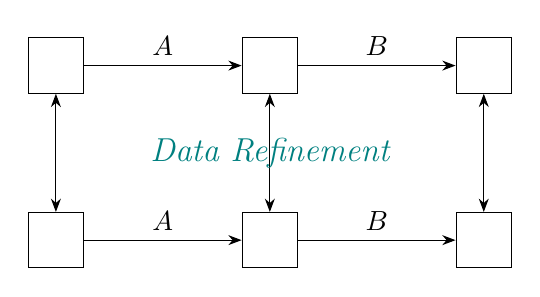
\begin{tikzpicture}[state/.style = {draw, rectangle, minimum size = 20pt},
  node distance = 1.5cm and 2.0cm, >=Stealth] 
  \node (1) [state] {};
  \node (2) [state, right = of 1] {};
  \node (3) [state, right = of 2] {};
  \path (1) edge[->] node [above] {$A$} (2)
	(2) edge[->] node [above] {$B$} (3);

  \node (11) [state, below = of 1] {};
  \node (22) [state, right = of 11] {};
  \node (33) [state, right = of 22] {};
  \path (11) edge[->] node [above] {$A$} (22)
	(22) edge[->] node [above] {$B$} (33);

  \foreach \u/\d in {1/11, 3/33} {
    \draw [<->] (\u) to (\d);
  }

  \draw [<->] (2) to node [align = center] {\textcolor{teal}{\it \large Data Refinement}} (22);
\end{tikzpicture}
\end{document}